\subsection{Differential-Mode \& Common-mode Gain}

The differential-mode gain and common-mode gain from simulations performed prior to this lab are approximately $20$ and $0.01$ \si{\volt}/\si{\volt}.
$v_{out(dm)}$ and $v_{out(cm)}$ can be found by evaluating the product of the corresponding gain values and input components.
Thus, $v_{out(dm)} = A_{dm}v_{in(dm)} = 4$\si{\volt} peak-to-peak and $v_{out(cm)} = A_{cm}v_{in(cm)} = 1$\si{\milli\volt} peak-to-peak.
However, the result for $v_{out(dm)}$ is much too large when compared to the amplitudes seen on the oscilloscope.
The result for $v_{out(cm)}$ is reasonable since the common-mode component of the output is typically a negligible quantity. \\

Using the results from the oscilloscope, and assuming that the common-mode component of the output is negligible, $v_{out(dm)}$ can be approximated by $V_{out+} - V_{out-} = 466$\si{\milli\volt} peak-to-peak.
The differential-mode gain can then be found: $A_{dm} = \frac{v_{out(dm)}}{v_{in(dm)}} = 2.33$ \si{\volt}/\si{\volt}.
This is significantly lower than the value from the simulation.
Because the common-mode output is assumed to be negligible, the common-mode gain cannot be conclusively found so the common-mode rejection ratio cannot be found either by extension.
However, if the common-mode gain from the simulation is assumed to be correct (this is a baseless assumption), then the CMRR would be $233$. \\

\subsection{Clamping \& Distortion}

Given the voltage ranges of which the amplifying transistors work from (\ref{fig:scope_7}) and (\ref{fig:scope_8}), $V_{out+}$ seems to exhibit a larger swing.
Although we biased these transistors as identically as we could with the current mirrors and DC voltage dividers, they still exhibit some differences.
Notably, the transistor for $V_{out+}$ clearly hits cutoff where the one for $V_{out-}$ does not.
The voltage variation in $V_{out+} - V_{out-}$ was earlier found to be 3.19\si{\volt}
Interestingly, this is approximately equal to $V_{DD} - V_{t}$, which is the normal limit to avoid distortion in voltage output for a common-source amplifier.
This indicates that although our input magnitude was quite large, it was not large enough to drive the transistors far enough into triode region to exhibit the maximum possible output swing of $V_{DD}$.
Since the gain in the triode region is so low, demonstrating that $V_{out+} - V_{out-}$ is at maximum 5V would require a very large input magnitude.

\FloatBarrier

\begin{figure}[h!]
	\centering
	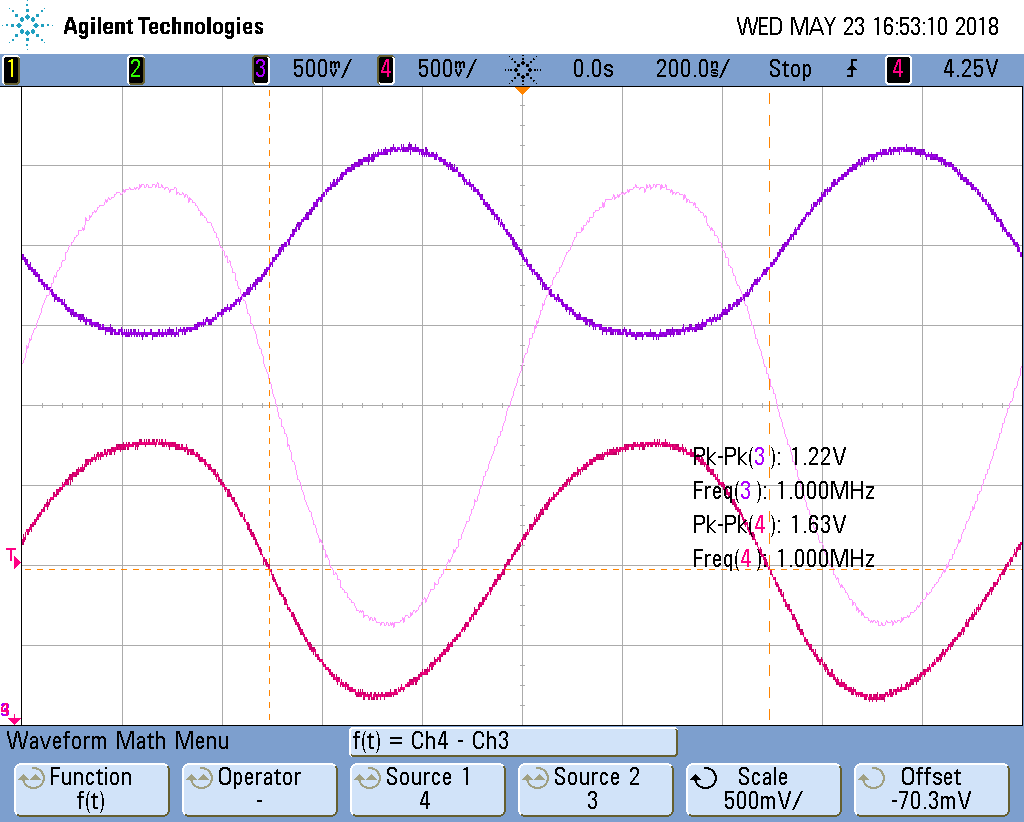
\includegraphics[scale=0.40]{./images/scope_6}
	\caption{Measured maximum signal swing of $V_{out+}$ and $V_{out-}$ from a 1.5\si{\volt} p/p input at 1MHz}
	\label{fig:scope_6}
\end{figure}

\FloatBarrier

Therefore, for this differential amplifier, the input signal magnitude should be no greater than 1.5V p/p to avoid significant distortion in signal.
This quantity is similar to the output voltage swing divided by $A_{dm}$.
